
\hypertarget{basic_configuration}{}
\section{Configuration}
\index{configuration}

This section provides information on Tinn-R configuration and associated
applications.


\subsection{Uninstall Tinn-R}
\index{installation}

\begin{itemize}
  \item \textbf{ALWAYS UNISTALL ANY PRIOR VERSION OF Tinn-R BEFORE
      INSTALLING A NEW ONE!} Tinn-R has its own uninstall option.
  \item The folder where Tinn-R project stores the ini files will
    not be removed when unistalling it. Why? Because whenever you
    install a different version all your preferences will be
    preserved.
  \item You can check where these files are located by checking
    \textit{Help/Ini files (path information)}. If you prefer,
    you may delete these settings by removing the entire folder manually.
    \textbf{All your preferences will be lost forever if you don't
      have a backup file}.
\end{itemize}


\hypertarget{basic_configuration_installconfigure}{}
\subsection{Install and configure Tinn-R and R}


\subsubsection{R basic configuration:}\\

\begin{itemize}
  \item Starting from version 1.18.X.X, \texttt{Tinn-R requires
      Rgui.exe to run in SDI mode}. So, Tinn-R is not compatible neither
    with Rgui.exe in MDI mode (only SDI) nor with S-PLUS. The
    latest compatible version was the historic 1.17.2.4.
  \item Starting from version 2.0.0.0, \texttt{Tinn-R requires
      \RR{} to run either Rterm.exe or Rgui.exe (in SDI mode)}.
  \item Starting from version 8.02.01.01, Rgui.exe must be launched from within Tinn-R so that it is properly
          identified at startup.
  \item You have three basic options in order to switch Rgui.exe from
    MDI to SDI:
    \begin{enumerate}
      \item In Rgui.exe, select \texttt{Edit/GUI preferences...},
        set SDI and click on \texttt{Save}, then \texttt{OK}
        without changing the name of the proposed file. Then,
        click \texttt{OK} or \texttt{Cancel} in the
        \texttt{Rgui.exe Configuration Editor} (ignore any eventual
        messages), and restart Rgui.exe (changes will not be taken
        into account in the current session).
      \item Manually edit the file \texttt{Rconsole}:
        \begin{Scode}
          ## Style
          # This can be yes (for MDI) or no (for SDI).
          MDI = no
        \end{Scode}
      \item Create a shortcut to \RR{} on your desktop (or anywhere that is convenient),
        and type in the switch \texttt{--sdi} after the \texttt{...$\backslash$Rgui.exe}
        in the \texttt{Target} box. To do this, right click on your shortcut, select
        \texttt{Properties} and navigate to the \texttt{Shortcut} tab.
    \end{enumerate}
\end{itemize}


\subsubsection{If you have any version of Tinn-R ($>$= 3.0.1.0) installed:}\\

If your version is the same or above 3.0.1.0, Tinn-R does not require any special configuration.
That is, the program is ready to be used. One important thing to be done before using it:
set a \RR{} mirror as close as possible to where you work. For that, first click on \texttt{CTRL + F8}.
This opens the \texttt{Tools} window, then click on \texttt{R/Mirrors}.
Select the \RR{} mirror and push the button that shows an hourglass in the taskbar.
The chosen repository will be the new default for all actions dependent repository
(install packages, upgrade packages, etc).


\subsubsection{If you have any version of Tinn-R ($<$= 2.2.0.2) installed:}\\

\begin{enumerate}
  \item Uninstall previous versions of Tinn-R
  \item Edit the file Rprofile.site (folder \textit{etc} where
    \RR{} is installed) and comment (or remove) all prior configuration
    scripts RELATED TO TINN-R
  \item Start \RR{}
  \item Install the following packages:
    \begin{enumerate}
      \item \href{http://cran.r-project.org/web/packages/TinnR/index.html}{TinnR}
      \item \href{http://cran.r-project.org/web/packages/svSocket/index.html}{svSocket}
      \item \href{http://cran.r-project.org/web/packages/formatR/index.html}{formatR}
    \end{enumerate}
  \item Close \RR{}
  \item Install the new version of Tinn-R
  \item Start Tinn-R
  \item From the Tinn-R main menu, choose the option
    \texttt{R/Configure/Permanent (Rprofile.site)}. It will write the
    following text to the file Rprofile.site:
    {\footnotesize
      {\color {darkred}
        \begin{verbatim}
          ##===============================================================
          ## Tinn-R: necessary packages and functions
          ## Tinn-R: >= 2.4.1.1 with TinnR package >= 1.0.3
          ##===============================================================
          ## Set the URL of the preferred repository, below some examples:
          options(repos='http://cran.at.r-project.org/')      # Austria/Wien
          #options(repos='http://cran-r.c3sl.ufpr.br/')       # Brazil/PR
          #options(repos='http://cran.fiocruz.br/')           # Brazil/RJ
          #options(repos='http://www.vps.fmvz.usp.br/CRAN/')  # Brazil/SP
          #options(repos='http://brieger.esalq.usp.br/CRAN/') # Brazil/SP

          library(utils)

          ## Check necessary packages
          necessary <- c('TinnR',
                         'svSocket',
                         'formatR')

          installed <- necessary %in% installed.packages()[, 'Package']
          if (length(necessary[!installed]) >=1)
          install.packages(necessary[!installed])

          ## Load packages
          library(TinnR)
          library(svSocket)

          ## Uncomment the two lines below if you want Tinn-R to always start R at start-up
          ## (Observation: check the path of Tinn-R.exe)
          #options(IDE='C:/Tinn-R/bin/Tinn-R.exe')
          #trStartIDE()

          ## Option
          options(use.DDE=T)

          ## Start DDE
          trDDEInstall()

          ## Short paths
          .trPaths <- paste(paste(Sys.getenv('APPDATA'),
                                  '\\Tinn-R\\tmp\\',
                                  sep=''),
                      c('',
                        'search.txt',
                        'objects.txt',
                        'file.r',
                        'selection.r',
                        'block.r',
                        'lines.r',
                        'reformat-input.r',
                        'reformat-output.r'),
                      sep='')
        \end{verbatim}
      } % color
    } % footnotesize
  \item Start Rgui.exe or Rterm.exe from within Tinn-R
  \item Read the content from the links below:
    \begin{itemize}
      \item \textit{\href{\#basic\_card}{Card}}: to know
        the shortcuts related with \RR{} and all others
      \item \textit{\href{\#whatisnew}{What is new}}:
        to know the news.
    \end{itemize}
\end{enumerate}


Information about how to customize the \texttt{Rprofile.site} file can be obtained from
\href{http://stat.ethz.ch/R-manual/R-patched/library/base/html/Startup.html}{Initialization at Start of an R Session}
and an example of this file from \href{http://sourceforge.net/p/tinn-r/news/?source=navbar}{SourceForge}.


\subsubsection{If you have any version of Tinn-R ($>$= 2.2.0.2) installed and configured:}\\

\begin{enumerate}
  \item Uninstall the prior version of Tinn-R 2.X.X.X
  \item Install the new version of Tinn-R
  \item Run it.
\end{enumerate}


\subsubsection{If you want to install any old version of Tinn-R ($<$= 2.0.0.0"):}\\

\begin{itemize}
  \item \textbf{Downgrading}: \texttt{rename (or delete) the folder
      where Tinn-R stores the ini files}. The uninstall is necessary
    since Tinn-R does not downgrade automatically. If you encounter
    any problems while downgrading, check the ini folder and respective
    files.
  \item Download and install Tinn-R.
  \item Install the \texttt{SciViews} bundle, then type
    \texttt{guiDDEInstall()} in \RR{} and \texttt{that's all}!

    \begin{footnotesize}
      \begin{verbatim}
        > install.packages('SciViews', dep=T)
        > guiDDEInstall()
      \end{verbatim}
    \end{footnotesize}

  \item Perhaps the best way to get \RR{} to communicate with
    Tinn-R from the time it is started is to add the
    following commands to \texttt{../etc/Rprofile.site}
    in the \RR{} install directory:

    \begin{Scode}
      #===============================================================
      # Tinn-R: necessary packages and functions
      #===============================================================
      library(utils)
      necessary = c('svIDE', 'svIO', 'svSocket', 'R2HTML')
      installed = necessary %in% installed.packages()[, 'Package']
      if (length(necessary[!installed]) >=1)
      install.packages(necessary[!installed], dep = T)

      library(svIDE)
      library(svIO)
      library(svSocket)
      library(R2HTML)
      guiDDEInstall()
    \end{Scode}

  \item If you chose the latter option \texttt{.../etc/Rprofile.site},
    a nice additional functionality is provided by adding the two
    lines below \texttt{BEFORE} the \texttt{library(svIDE)} command:

    \begin{Scode}
      options(IDE = 'C:/Tinn-R/bin/Tinn-R.exe')
      options(use.DDE = T)
    \end{Scode}

    The first line tells \RR{} that you want to use Tinn-R as your IDE (Integrated
    Development Environment).  To make this happen, you should change the path
    that leads to where \texttt{Tinn-R.exe} is installed if it happens to be
    different from the default configuration. The second line indicates that
    you want to start the DDE server automatically.

    By doing this, Tinn-R will start automatically once you invoke \RR{}.
\end{itemize}


\subsection{Rgui.exe}
\index{Rgui}


\includegraphics[scale=0.50]{./res/focus.png}

\begin{itemize}
  \item Tinn-R has an icon within the \textit{Options toolbar}
    containing the hint \texttt{Options: return focus to editor
      after send/control Rgui.exe} which enables the user to configure
    the focus control. When \texttt{checked}:
    \begin{itemize}
      \item If the editor has the focus: it will \texttt{go back}
        to the editor after any \textit{send to} or \textit{R control}
        action;
      \item Otherwise, the focus will be set to the Rgui.exe interface.
    \end{itemize}
\end{itemize}


\subsection{Rterm.exe}
\index{Rterm}

\begin{itemize}
  \item The above-mentioned icon will be disabled with Term interface.
    The following will then happen:
    \begin{itemize}
      \item If the focus is placed on the editor it will \texttt{go back}
        to the editor after any \textit{send to} or \textit{R control} action;
      \item If the focus is placed on the Term (\textit{IO} or \textit{LOG}),
        it will be \texttt{maintened} in this interface (\textit{IO});
      \item Situations above are also the case when working with two monitors.
    \end{itemize}
\end{itemize}


\newpage
\subsection{Term interface and debug package}
\index{debugging}

\begin{itemize}
  \item Several changes were made to the debug package (1.0.2) regarding
    the messaging system (\textit{stdout} and \textit{stderr}). The
    default option is no longer compatible with Term interface
    implementation.
  \item The best way to make it compatible again is to add the option
    below to the Rprofile.site file:

    \begin{footnotesize}
      \begin{verbatim}
        options(debug.catfile = 'stdout')
      \end{verbatim}
    \end{footnotesize}

   \item This option is automatically sent to the \RR{} interpreter from version 3.0.3.0 of Tinn-R project.
\end{itemize}


\hypertarget{configuration_spellerinstalation}{}
\subsection{Speller installation}
\index{speller}

\begin{itemize}
  \item To install this resource:
    \begin{enumerate}
      \item Close Tinn-R (if it is running);
      \item Download the
        \href{http://www.luziusschneider.com/Speller/English/index.htm}{dictionaries}
        you would like to add to Tinn-R;
      \item Install the file (for example ISpEnFrGe.exe);
    \end{enumerate}
  \item Upon start, Tinn-R will recognize all installed dictionaries.
    You should choose one as your default.
  \item Before installing new dictionaries, it is strongly
    recommended that you close Tinn-R.
  \item Another useful tool is the \texttt{UserDicEditor} which
    enables the editing of dictionaries.
\end{itemize}


\subsection{Inverse DVI search}
\index{inverse DVI search}
\index{search!inverse DVI }
\index{DVI!inverse search}

\begin{itemize}
  \item Tinn-R is able to perform \texttt{inverse DVI search}. To get this
    function to work, include in your DVI previewer the path of the
    binary executable file for Tinn-R along with the parameters for
    file and line.  For example, using YAP under Miktex, the configuration
    would be (assuming a default path for Tinn-R):
    \index{Miktex}

    \begin{footnotesize}
      \begin{verbatim}
        C:\Tinn-R\bin\Tinn-R.exe "%f;%l"
        
        Note:
        %f: file
        %l: line
      \end{verbatim}
    \end{footnotesize}

    \begin{itemize}
      \item Please make sure that there is no space between the
        parameters \%f(related to file) and \%l(related to line);\\\\
        \includegraphics[scale=0.50]{./res/yap_01.png}~~
        \includegraphics[scale=0.50]{./res/yap_02.png}\\
      \item It is necessary to add the parameter for \TeX~Live or Mik\TeX~compilation
        within Tinn-R (\textit{Options/Application/Processing/Latex/DVI}):
        latex -c-style-errors \texttt{--src-specials};

        \begin{footnotesize}
          \begin{verbatim}
            latex -c-style-errors --src-specials
            and
            bibtex --src-specials
          \end{verbatim}
        \end{footnotesize}

        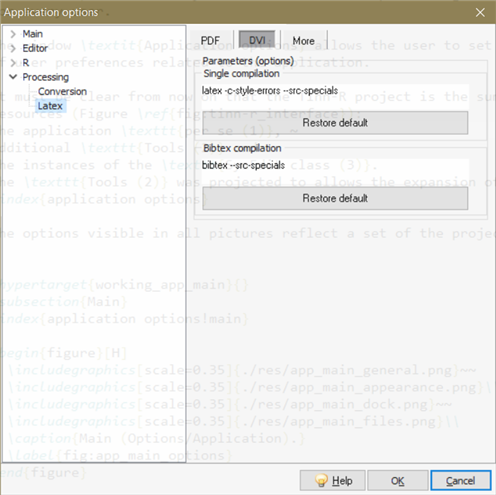
\includegraphics[scale=0.50]{./res/app_processing_latex_dvi.png}\\
    \end{itemize}
\end{itemize}


\subsection{Inverse PDF search}
\index{inverse PDF search}
\index{search!inverse PDF}
\index{PDF!inverse search}

\begin{itemize}
  \item Tinn-R is able to perform \texttt{inverse PDF search}. To get this
    function to work, include in your PDF previewer (we recomend Sumatra) the path of the
    binary executable file for Tinn-R along with the parameters for
    file and line.  For example, using Sumatra, the configuration
    would be (assuming a default path for Tinn-R):
    \index{Sumatra}

    \begin{footnotesize}
      \begin{verbatim}
        C:\Tinn-R\bin\Tinn-R.exe "%f;%l"
        
        Note:
        %f: file
        %l: line
      \end{verbatim}
    \end{footnotesize}

    \begin{itemize}
      \item Please make sure that there is no space between the
        parameters \%f(related to file) and \%l(related to line);\\\\
        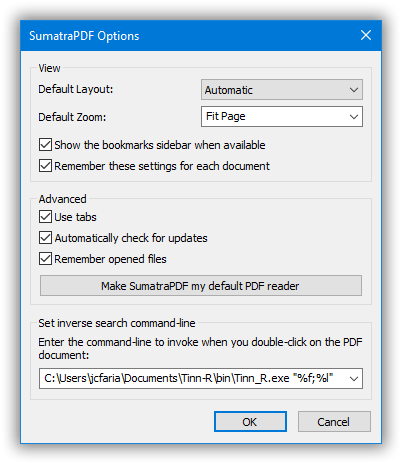
\includegraphics[scale=0.80]{./res/sumatra.png}\\
      \item It is necessary to add the parameter for Miktex compilation
        within Tinn-R (\textit{Options/Application/Processing/Latex/PDF}):
        pdflatex -c-style-errors \texttt{ --synctex=1};
      \item Tinn-R can do all of this automatically by setting the
        option \textit{Restore default}:

        \begin{footnotesize}
          \begin{verbatim}
            pdflatex -c-style-errors --synctex=1
            and
            bibtex
          \end{verbatim}
        \end{footnotesize}

        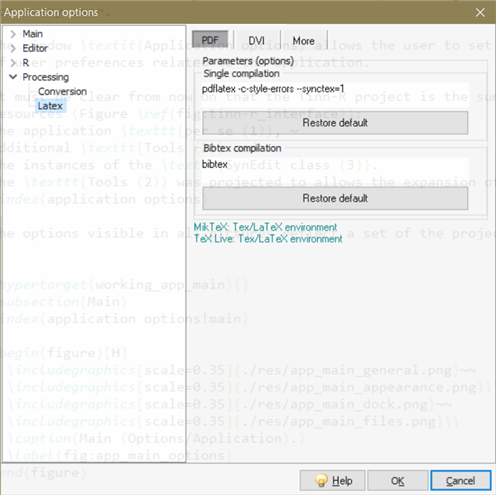
\includegraphics[scale=0.60]{./res/app_processing_latex_pdf.png}\\
    \end{itemize}
\end{itemize}


\subsection{Ruby and Deplate}
\index{Ruby}
\index{Deplate}

\begin{itemize}
  \item \href{http://deplate.sourceforge.net/}{Deplate}
    \href{http://deplate.sourceforge.net/deplate.html}{(user guide here)}
    is a remote
    \href{http://www.ruby-lang.org/en/}{Ruby} based tool for
    converting documents written in wiki-like markup to \LaTeX, HTML, HTML slides,
    or DocBook format. Deplate supports page templates, embedded \LaTeX ~code,
    footnotes, citations, bibliographies, automatic generation of indices, tables
    of contents, among others. Deplate can also be used to create Web pages and,
    via \LaTeX ~or DocBook, high-quality printouts.

  \item Tinn-R works with the Ruby interpreter for Windows (ruby.exe) and Ruby
    scripts to generate file conversation within deplate.

  \item To install and configure these resources follow these steps:
    \begin{enumerate}
      \item Download and unzip the
        \href{http://www.ruby-lang.org/en/}{Ruby}
        interpreter anywhere in your computer;
      \item Download and unzip
        \href{http://deplate.sourceforge.net/Download.php}{Deplate}
        anywhere in your computer;
      \item Within Tinn-R, go to \texttt{Options/Application/Processing/Conversion/Deplate}
        and add information on parameters (\texttt{-f} is the default),
        the interpreter path (\texttt{ruby.exe}), and the converter
        (\texttt{deplate.rb ruby script});\\

        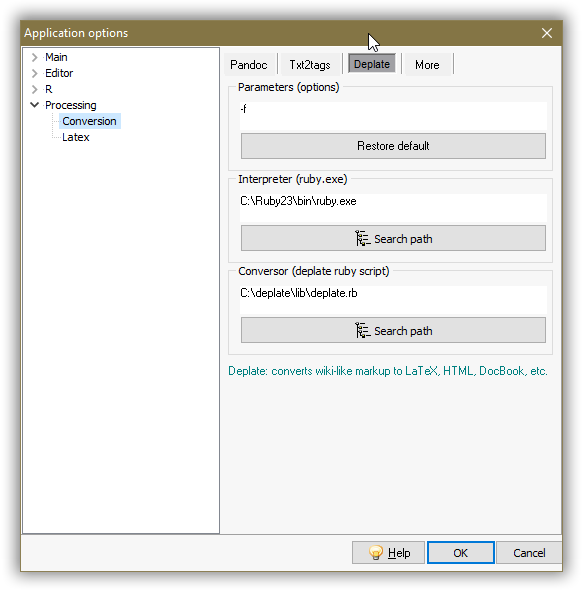
\includegraphics[scale=0.50]{./res/app_processing_conversion_deplate.png}\\
    \end{enumerate}
\end{itemize}

The conversion options using \texttt{Deplate} depends of the file extension.
Are recognized: \texttt{.dp, .dpt, .dplt, .deplate and .txt}.

We recently observed a problem when converting files with file names with an
underscore. For example \texttt{deplate\_intro.dplt}. In these cases the file
conversion is completed, but Tinn-R won't open the file since it can't find it.
This pattern is caused by Deplate (a ruby script) generating a file named
\texttt{deplate\_\_intro.html}. \textit{Observe that this file name contains a
double underscore}. In sum, for the time being, avoid underscores in file
names when you intend to convert them later through Deplate.


\subsection{Pandoc}
\index{Pandoc}

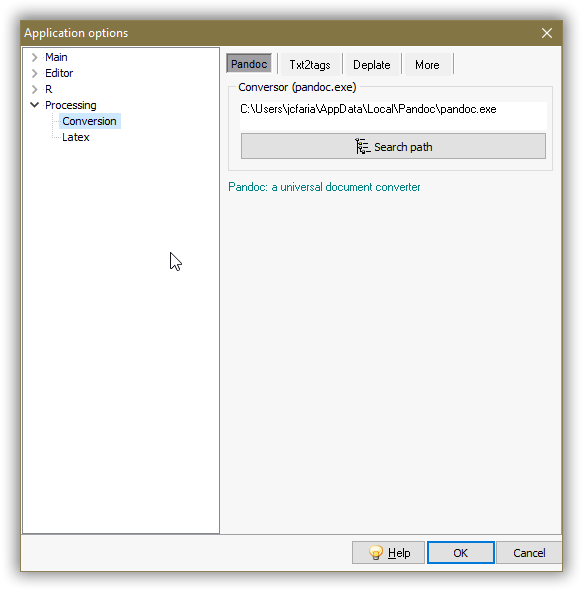
\includegraphics[scale=0.50]{./res/app_processing_conversion_pandoc.png}

\begin{itemize}
\item If you need to convert files from one markup format into another, \href{http://johnmacfarlane.net/pandoc/index.html}{Pandoc} is your swiss-army knife.
\item To install and configure Pandoc resources, just follow these steps:
 \begin{enumerate}
 \item \href{http://code.google.com/p/pandoc/downloads/list}{Download} and install the converter Pandoc anywhere in your computer;
 \item Within Tinn-R, go to \texttt{Options/Application/Processing/Conversion/Pandoc} and add information on path (\texttt{pandoc.exe}).

 \end{enumerate}
\item Pandoc can \href{http://johnmacfarlane.net/pandoc/README.html}{convert} documents:
\end{itemize}

\begin{footnotesize}\begin{tabularx}{130pt}{lX} \\
\hline
\textbf{From} \\
\hline
  DocBook \\
  HTML \\
  JSON version of native AST \\
  \LaTeX \\
  markdown \\
  native Haskell \\
  reStructuredText \\
  textile \\
\hline
\end{tabularx}\end{footnotesize}

\begin{footnotesize}\begin{tabularx}{\textwidth}{>{\hsize=0.4\hsize}X>{\hsize=0.7\hsize}X} \\
    \hline
    \textbf{To} & \textbf{Subset(s)} \\
    \hline
    Documentation formats & DocBook, GNU TexInfo, Groff man pages \\
    Ebooks & EPUB \\
    HTML formats & XHTML, HTML5, and HTML slide shows using Slidy, Slideous, S5, or DZSlides \\
    Lightweight markup formats & Markdown, reStructuredText, AsciiDoc, MediaWiki markup, Emacs Org-Mode, Textile \\
    PDF via \LaTeX \\
    TeX formats & \LaTeX, ConTeXt, \LaTeX Beamer slides \\
    Word processor formats & Microsoft Word docx, OpenOffice/LibreOffice ODT, OpenDocument XML \\
    \hline
  \end{tabularx}\end{footnotesize}


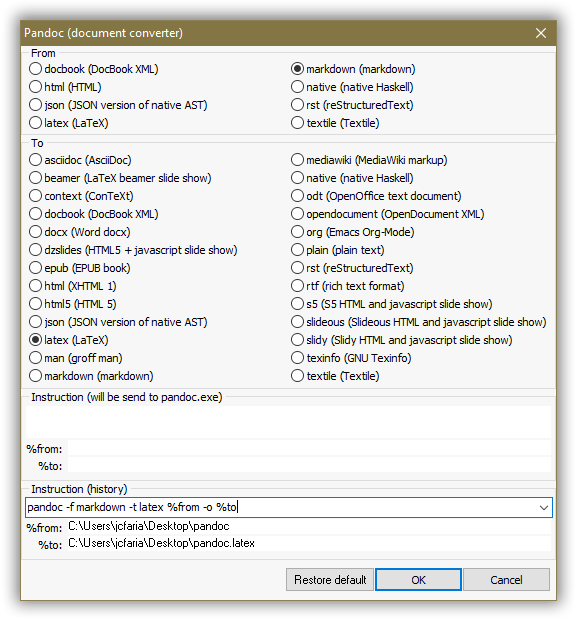
\includegraphics[scale=0.50]{./res/pandoc.png}

\subsection{Python and Txt2tags}
\index{Python}
\index{Txt2tags}

\begin{itemize}
  \item \href{http://txt2tags.sourceforge.net}{Txt2tags}
    \href{http://txt2tags.sourceforge.net/userguide}{(user guide here)}
    converts a text file with \texttt{minimal and human readable markup} to:
    HTML, XHTML, SGML, \LaTeX, Lout, UNIX man page, Wikipedia, Google Code Wiki,
    DokuWiki, MoinMoin, MagicPoint (mgp), and PageMaker. It is simple and fast,
    featuring automatic TOC, macros, filters, include, tools, GUI, CLI,
    Web interfaces, translations, and extensive documentation.

  \item Tinn-R works with the Phyton interpreter for Windows (python.exe), using
    Python scripts to make the conversion (txt2tags).

  \item To install and configure Python resources, just follow these steps:
    \begin{enumerate}
      \item Download and install the
        \href{http://www.python.org/download/}{Python}
        interpreter anywhere in your computer;
      \item Download and unzip
        \href{http://txt2tags.sourceforge.net/}{Txt2tags}
        anywhere in your computer;
      \item Within Tinn-R, go to \texttt{Options/Application/Processing/Txt2tags}
        and add information on parameters (\texttt{-t} is the default),
        interpreter path (\texttt{python.exe}) and the
        converter (\texttt{txt2tags python script});\\

        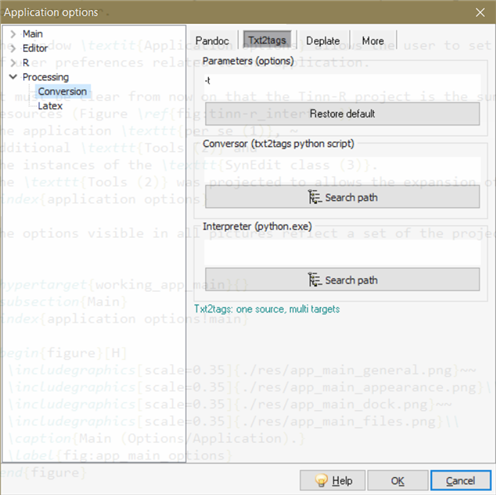
\includegraphics[scale=0.50]{./res/app_processing_conversion_txt2tags.png}\\
    \end{enumerate}
\end{itemize}

The conversion options using \texttt{Txt2tags} depends of the file extension.
Are recognized: \texttt{.t2, .t2t, .txt2tags. and .txt}.
